\documentclass[tikz, margin=3mm]{standalone}
\usepackage{amsmath,amsfonts,tikz,fontspec}
\usetikzlibrary{arrows.meta, bending, positioning}

\setmainfont{DejaVu Serif}
\setsansfont{DejaVu Sans}

\newcommand{\mathng}{{\text{\normalfont \textit{ŋ}}}}

\newcommand{\txtop}[1]{\mathop{\mathrm{#1}}\limits}
\newcommand{\argmin}{\txtop{argmin}}
\newcommand{\MSE}{\txtop{MSE}}
\newcommand{\ntos}{\txtop{noise2self}}
\newcommand{\PCA}{\txtop{PCA}}
\newcommand{\kNN}{\txtop{kNN}}
\newcommand{\WAK}{\txtop{WAK}}
\newcommand{\leiden}{\txtop{leiden}}
\newcommand{\rdim}{\txtop{reducedimension}}


\begin{document}

      \noindent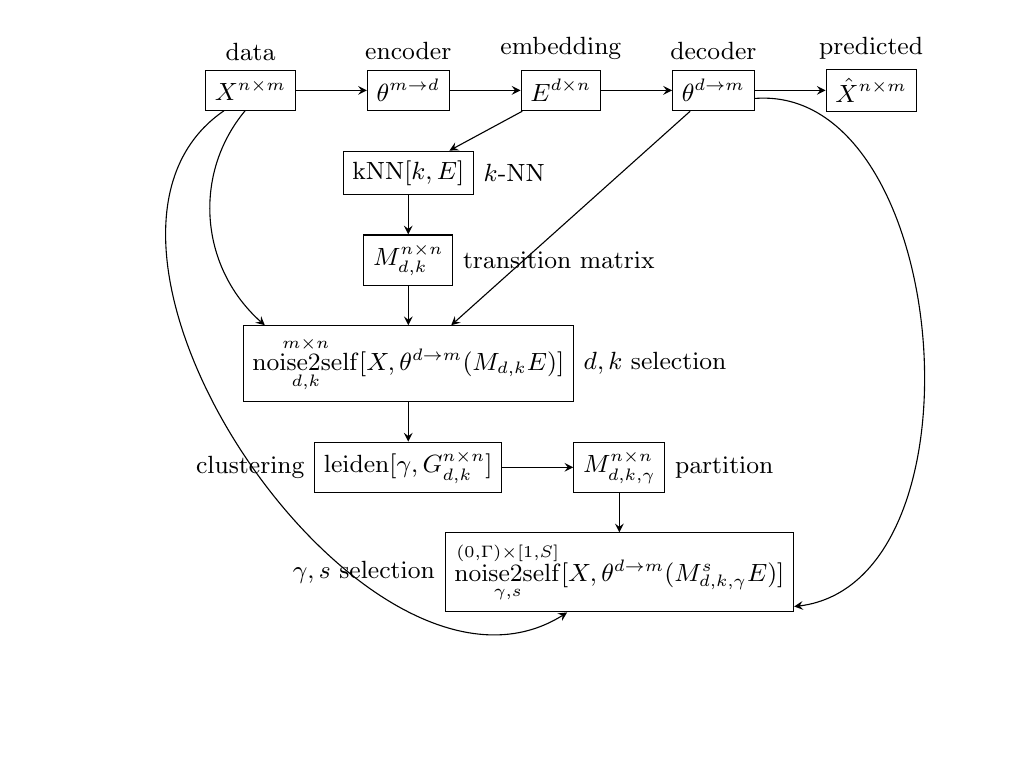
\begin{tikzpicture}[
        node distance = 5mm and 9mm,
        punkt/.style = {rectangle, draw},
        pil/.style = {black, -stealth},
        font=\small
        ]
        \node[punkt,label=above:data] (X) {$X^{n \times m}$};
        \node[punkt,label=above:encoder] (encoder) [right=of X] {$\theta^{m \to d}$};
        \node[punkt,label=above:embedding] (E) [right=of encoder] {$E^{d \times n}$};
        \node[punkt,label=above:decoder] (decoder) [right=of E] {$\theta^{d \to m}$};
        \node[punkt,label=above:predicted] (Xhat) [right=of decoder] {$\hat{X}^{n \times m}$};
        \node[punkt,label=right:$k$-NN] (knn) [below=of encoder] {$\kNN[k,E]$};
        \node[punkt,label=right:transition matrix] (G) [below=of knn] {$M_{d,k}^{n \times n}$};
        \node[punkt,label=right:{$d,k$} selection] (ksel) [below=of G] {$\ntos_{d,k}^{m \times n}[X,\theta^{d \to m}(M_{d,k}E)]$};
        \node[punkt,label=left:clustering] (leiden) [below=of ksel] {$\leiden[\gamma,G_{d,k}^{n \times n}]$};
        \node[punkt,label=right:partition] (P) [right=of leiden] {$M_{d,k,\gamma}^{n \times n}$};
        \node[punkt,label=left:{$\gamma,s$} selection] (gammasel) [below=of P] {$\ntos_{\gamma,s}^{(0,\Gamma)\times[1,S]}[X,\theta^{d \to m}(M_{d,k,\gamma}^sE)]$};
        
        \draw[pil] (X) edge (encoder)
        (encoder) edge (E)
        (E) edge (decoder)
        (decoder) edge (Xhat)
        (E) edge (knn)
        (knn) edge (G)
        (G) edge (ksel)
        (X) edge[bend right=45] (ksel)
        (decoder) edge (ksel)
        (ksel) edge (leiden)
        (leiden) edge (P)
        (P) edge (gammasel)
        (X) edge[bend right=90] (gammasel)
        (decoder) edge[bend left=90] (gammasel);
        
      \end{tikzpicture}
      \end{document}
